\section{Thermoelastic cube (3D)}
\subsection{Definition}
The problem given in section \ref{sec:tm2d} for plane strain conditions is considered in a 3D model. 
Initial and boundary conditions are similar to that described in section \ref{sec:tm2d}.
Material properties are given in Table \ref{tab:tm2D}. 
Results of the 3D model are compared with that of the 2D model.

\subsection{Solution}
%\subsubsection{Analytical solution}
%\subsubsection{Numerical solution}
Numerical simulation is conducted with a 3D model obtained by extruding the 2D model in off-plane direction for 1 unit.
The domain is discretized into hexahedra (Figure \ref{fig:TM3Mesh}).

\begin{figure}[!htb]
\centering
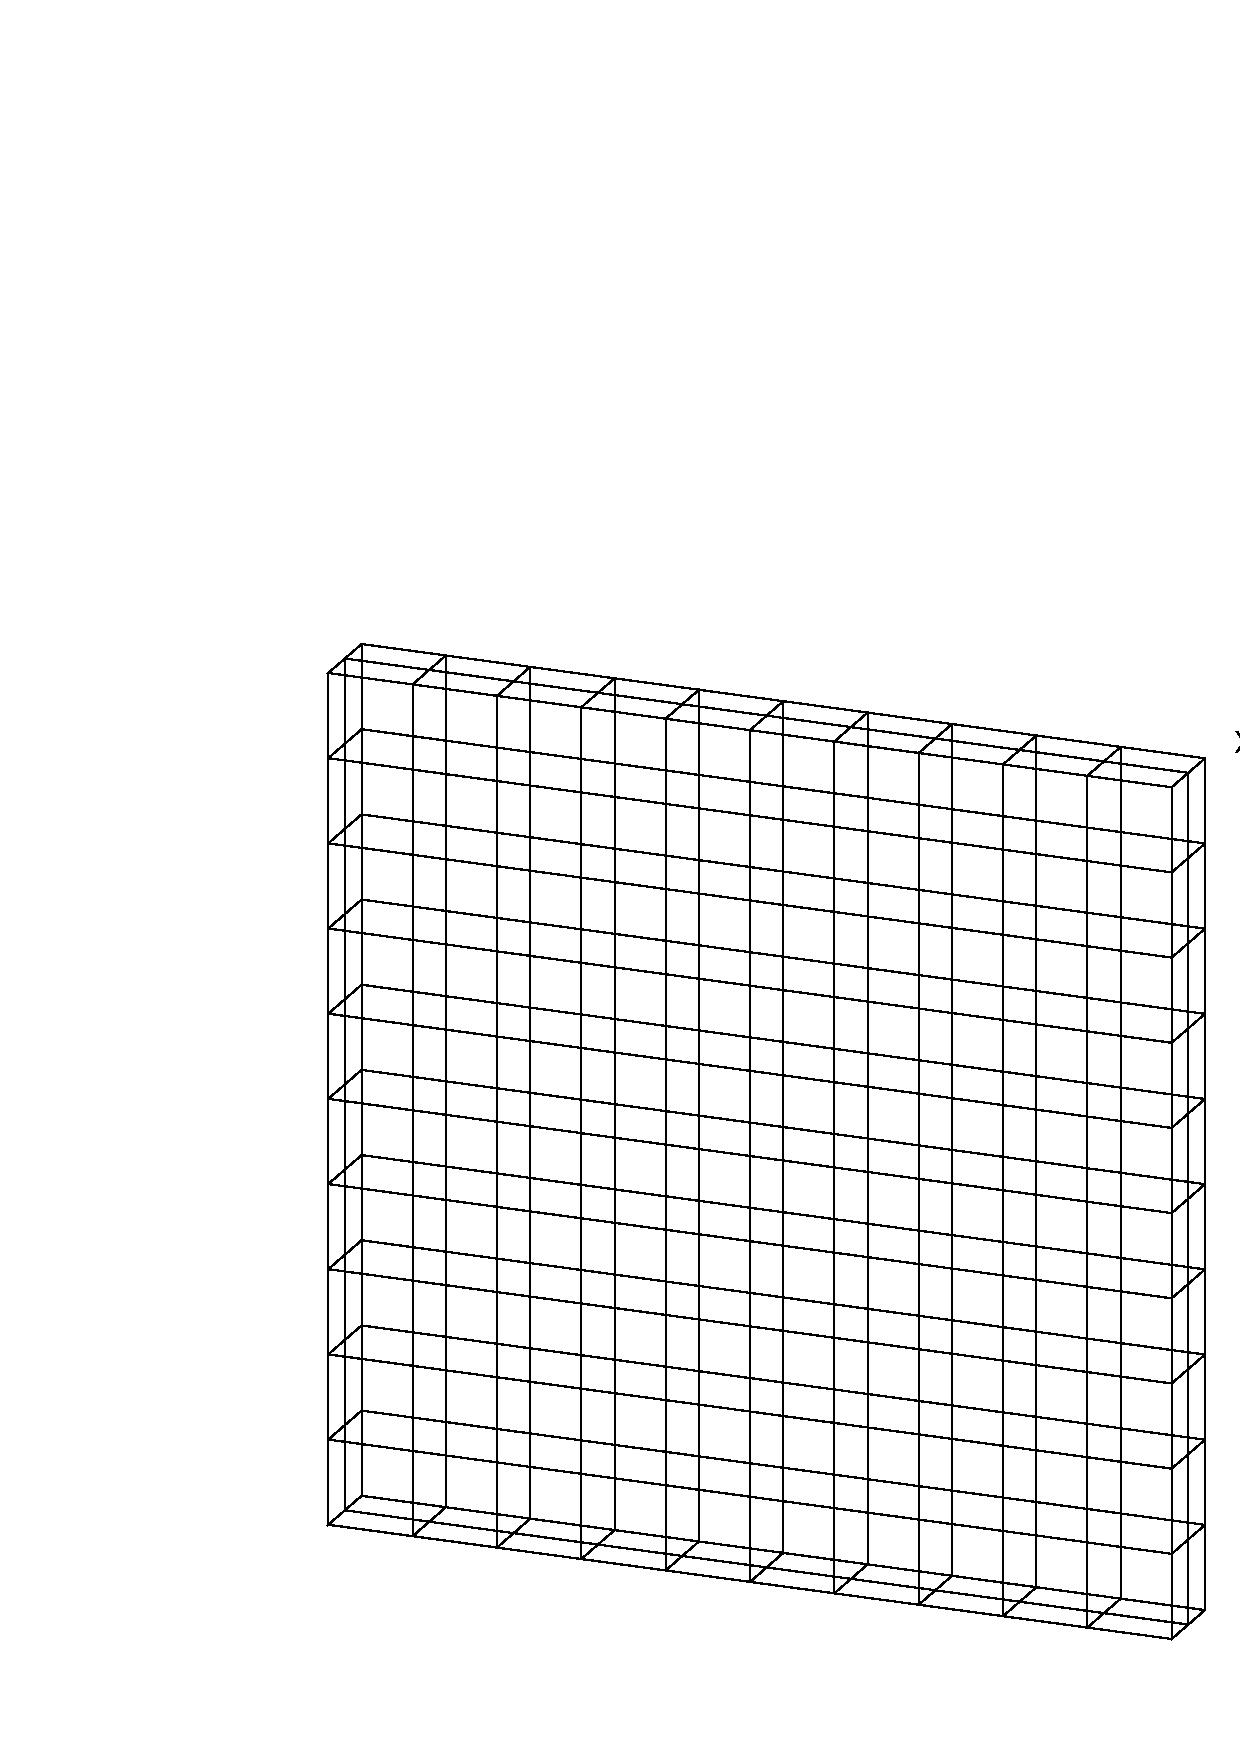
\includegraphics[height=5cm]{PART_III/TM/figures/3D_mesh}\\
\caption{Mesh for TM coupling 3D problem }
\label{fig:TM3Mesh}
\end{figure}



\subsection{Results}
Figure \ref{fig_TM2_r} provides the distribution of temperature and vertical stress after 100 time steps.
The distribution is identical to that given in Figure \ref{fig_TM1_r} for plane strain problem.
Figure \ref{fig:TMcmp} gives a comparison about the variation of state variables at the gravity center of 2D and 3D model.
 The results agree well with each other.

\begin{figure}[!htbp]
\begin{center}
\epsfig{figure=PART_III/TM/figures/3D_T,height=6cm}
\epsfig{figure=PART_III/TM/figures/3D_szz,height=6cm}
\end{center}
\caption{Distribution of temperature and vertical stress}
\label{fig_TM2_r}
\end{figure}

\begin{figure}[!htbp]
\centering
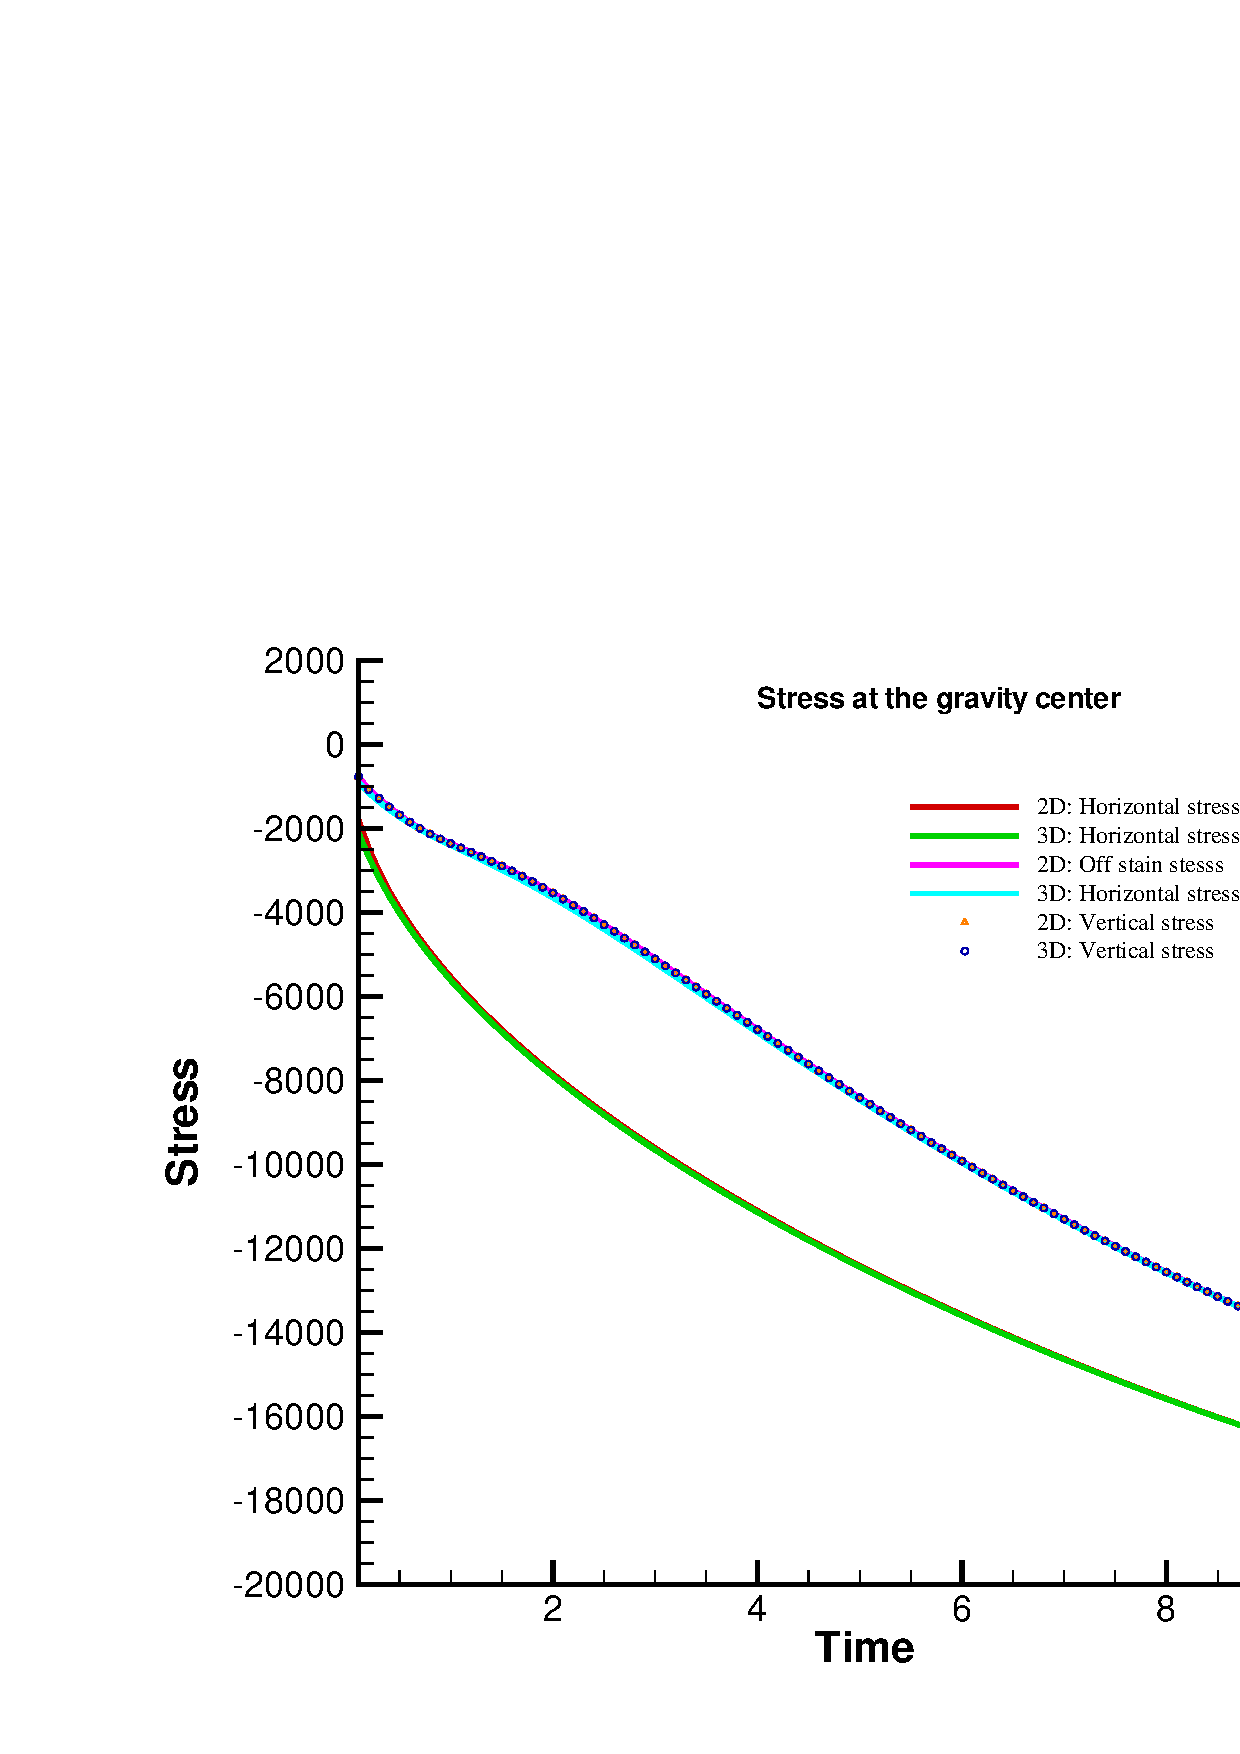
\includegraphics[height=7cm]{PART_III/TM/figures/2D_3D_cmp}\\
\caption{Comparison of 2D, 3D results }
\label{fig:TMcmp}
\end{figure}
